\chapter{VideoConferencia usando WebRTC}
\section{Enunciado}
Las aplicaciones multimedia en tiempo real permiten conectar a distintos usuarios a través de la red e intercambiando información y contenido de  audio, vídeo. Un ejemplo de este tipo de aplicación es Skype que ha tenido mucho éxito ya que permite a sus usuarios establecer videollamadas e intercambiar información una vez se haya instalado el software.
\begin{figure}[!h]
\begin{center}
   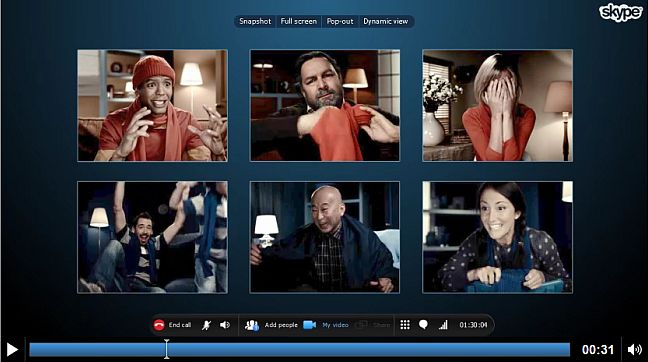
\includegraphics[width=0.5\linewidth]{Figures/skype}
	\decoRule
	\caption[Ejemplo sitio Web]{Skype interfaz videollamada.}
\label{fig:canvasPrimitivas}
\end{center}
\end{figure}

En esta ultima practica se pide desarrollar una aplicación web similar a Skype que permita a los usuarios conectarse entre si a través de la url de la aplicación.
\paragraph{Requisitos}
Los usuario dentro de la aplicación podrán seleccionar los elementos multimedia (audio y vídeo) que desean compartir y se les permitirá seleccionar o crear una sala donde realizar la videoconferencia. Dentro de la sala dispondrán de un chat y la opción de intercambiar ficheros por medio de WebRTC.

Como mecanismo adicional sera necesario el desarrollo de un servidor de señalización para la fase de comunicación inicial de WebRTC.
\paragraph{Tecnologías}
En el desarrollo de la practica es necesario/obligatorio que se haga uso de las tecnologías que se listan a continuación:
\begin{enumerate}
    \item WebRTC
    \item API File
    \item NodeJS
    \item WebSockets
    \item Boostratps
\end{enumerate}
\section{Diseño}
La figura \ref{fig:ComunnicacionWebRTC} muestra el esquema utilizado en el desarrollo de esta practica. Contiene cada uno de los elementos que intervienen desde el proceso de señalización hasta que se convierte en una comunicación Peer-to-Peer.
\begin{figure}[!h]
\centering
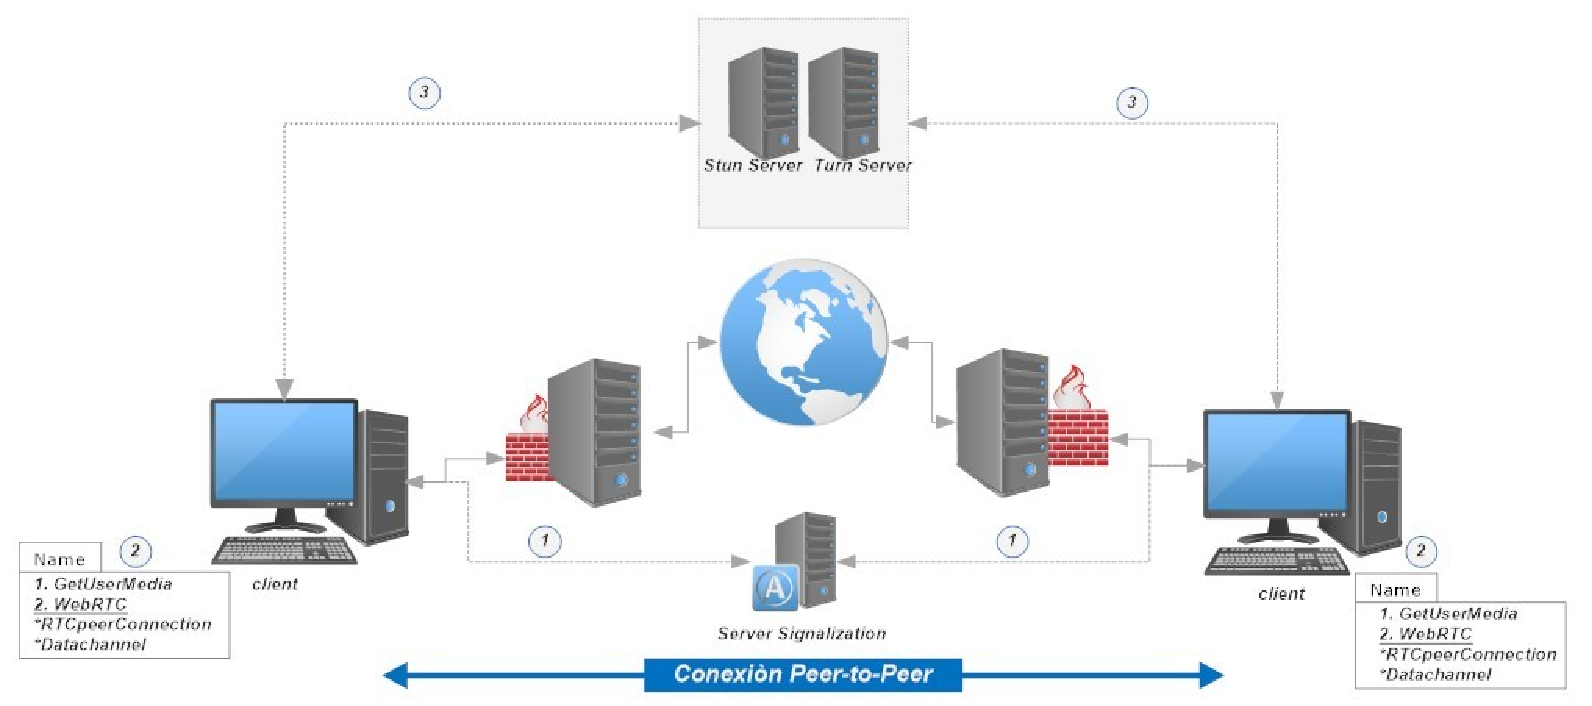
\includegraphics[width=0.9\linewidth]{Figures/ComunnicacionWebRTC}
\decoRule
\caption[Creación oferta cliente.]{Creación oferta cliente.}
\label{fig:ComunnicacionWebRTC}
\end{figure}

La topología que se establece entre lo usuarios dentro de una sala en la comunicacion Peer-To-Peer se  indica en la figura \ref{fig:Coneccion_finish}.
\begin{figure}[!h]
\centering
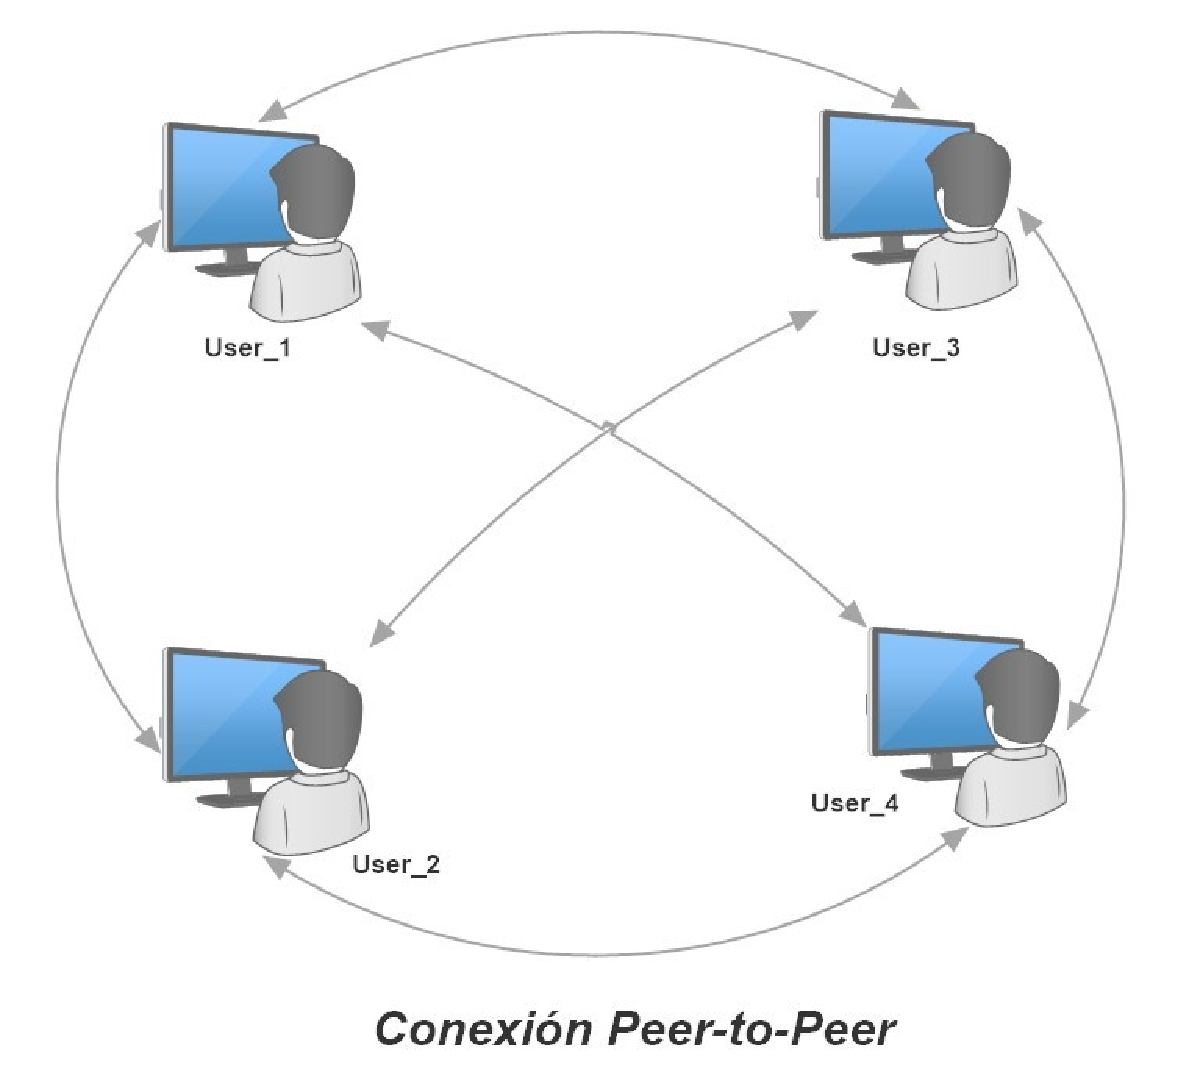
\includegraphics[width=0.3\linewidth]{Figures/Conexcion_finish}
\decoRule
\caption[Conexión Peer-to-Peer final.]{Conexión Peer-to-Peer final.}
\label{fig:Coneccion_finish}
\end{figure}


%%%%%%%% Servidor Desarrollo %%%%%%%%
\section{Desarrollo Servidor Señalización}
Para crear el servidor nos apoyamos en las librería \texttt{node-static}, \texttt{http} y \texttt{socket.io}. La figura \ref{fig:EjecucionServer} muestra al servidor encendido con la instancia de WebSocktes operativa.
\begin{lstlisting}[
caption=Creación Servidor de Señalizacion.]
 var static = require('node-static');
 var http = require('http');
 var file = new(static.Server)();
 var app = http.createServer(function (req, res) {
  file.serve(req, res);
 }).listen(8181);
 var io = require('socket.io').listen(app);
\end{lstlisting}
%\begin{figure}[!h]
%\begin{center}
%   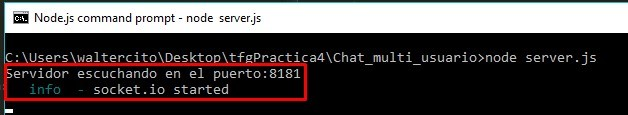
\includegraphics[width=0.65\linewidth]{Figures/InicioServidor}
%	\decoRule
%	\caption[ServidorSeñalizacion]{Ejecución Servidor de Señalizacion APP.}
%\label{fig:EjecucionServer}
%\end{center}
%\end{figure}

El tareas que realiza el servidor se divide en Inicio de Conexión y Mensajes señalización WebRTC que explicamos en detalle a continuación. 
\subsection*{Inicio de conexión}
Esta etapa se encarga de gestionar el acceso de los usuarios en una sala de la aplicación.  Se define el evento \texttt{InfoRoom} que envía un mensaje \texttt{ReplayInfoRoom} con la lista de salas existentes.
\begin{lstlisting}[,
caption=Request/Replay lista de salas existentes.]
 socket.on('infoRoom',function() {
  socket.emit('ReplayInfoRoom',listRooom);
 });
\end{lstlisting}
La figura \ref{fig:EjecucionInfoRoom} muestra como el servidor realiza el envió de este mensaje.
\begin{figure}[!h]
\begin{center}
   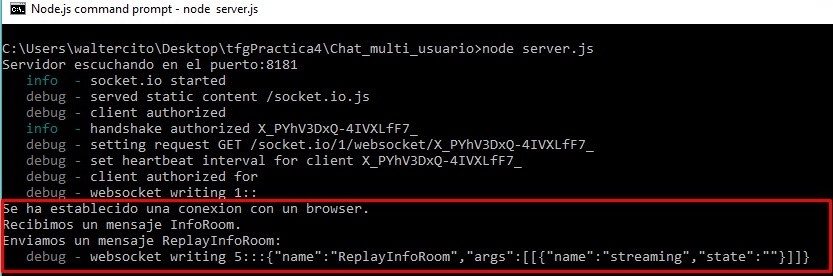
\includegraphics[width=0.8\linewidth]{Figures/InfoRoomServer}
	\decoRule
	\caption[Request/Replay Salas Servidor]{Request/Replay lista de salas del Servidor.}
\label{fig:EjecucionInfoRoom}
\end{center}
\end{figure}

Además define el evento \texttt{Stablish\_connect} para obtener el nombre del usuario y el de sala a la que el usuario quiere acceder. Con el nombre de la sala comprueba su existencia por medio de la función \texttt{getRoom(nameRoom)} en caso de no existir la guarda en la lista de salas y finaliza comprobando que la sala no este llena. Finaliza envíando un mensaje \texttt{CreateStream} con el identificador de conexión y un mensaje \texttt{NewJoined} al resto de usuario de la sala para que conozcan la existencia del nuevo miembro.
\begin{lstlisting}[
caption=Request/Replay del establecimiento de conexion.]
 socket.on('stablish_connection',function(name,room){
  if(!getRoom(room)){
    setRoom(room,'');
  };
  var numClients = io.sockets.clients(room).length;
  if(numClients < 3){
   socket.username = name;
   socket.room =room;
   socket.join(room);
   socket.emit('CreateStream',socket.id);
   socket.broadcast.to(room).emit('New_Joined',socket.id);
  }else{
   socket.emit('RejectStream',socket.id);
  }
 });
\end{lstlisting}
La figura \ref{fig:EjecucionStablishConnection} muestra como el servidor realiza el envió de este mensaje.
\begin{figure}[!h]
\begin{center}
   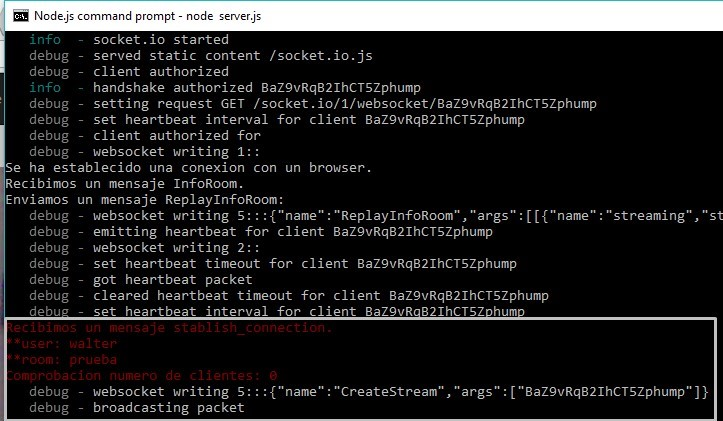
\includegraphics[width=0.9\linewidth]{Figures/StablishConnectionServer}
	\decoRule
	\caption[Request/Replay conexión Servidor]{Request/Replay conexión al Servidor.}
\label{fig:EjecucionStablishConnection}
\end{center}
\end{figure}

\subsection*{Mensajes señalización WebRTC}
El momento en que se quiere establecer la conexión WebRTC el servidor tiene como función encaminar los mensajes entre los participantes de la conexión. Cada uno de los mensajes de señalización viajan dentro del mensaje \texttt{message} por lo que se crea un evento con este nombre que consulta el id destino para encaminar el mensaje correctamente.
\begin{lstlisting}[
caption=Mensajes de señalizacion.]
 socket.on('message',function(message,room){
  io.sockets.socket(message.id_dest).emit('message', message);
 });
\end{lstlisting}

La figura \ref{fig:AnswerServer} encamina la oferta, la figura \ref{fig:OfferServer} encamina la respuesta y la figura \ref{fig:IceCandidateVideos} encamina los IceCandidate.
\begin{figure}[!h]
\begin{center}
   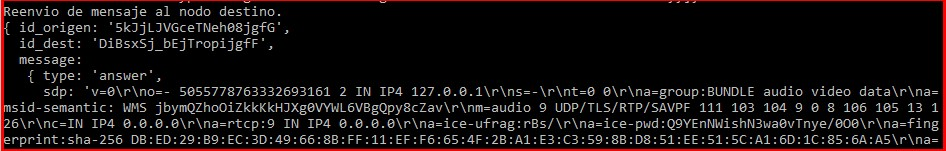
\includegraphics[width=1\linewidth]{Figures/AnswerServer}
	\decoRule
	\caption[Mensaje señalización Answer.]{Mensaje Answer.}
\label{fig:AnswerServer}
\end{center}
\end{figure}
\begin{figure}[!h]
\begin{center}
   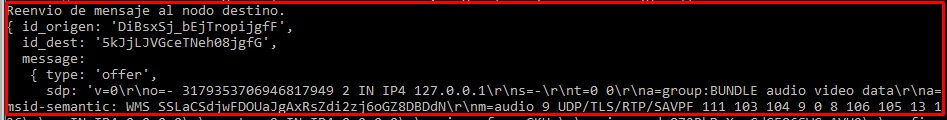
\includegraphics[width=1\linewidth]{Figures/OfferServer}
	\decoRule
	\caption[Mensaje señalización Offer.]{ Mensaje Offer.}
\label{fig:OfferServer}
\end{center}
\end{figure}
\begin{figure}[!h]
\begin{center}
   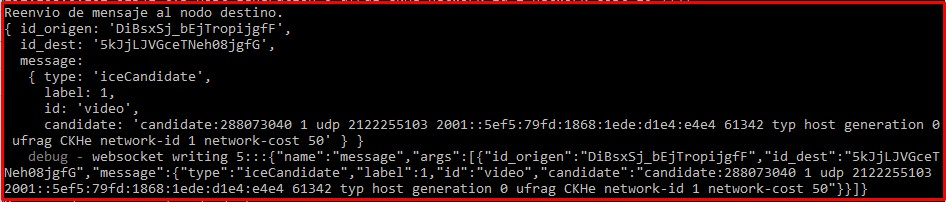
\includegraphics[width=1\linewidth]{Figures/IceCandidateVideos}
	\decoRule
	\caption[Mensaje señalización Icecandidate.]{ Mensaje Icecandidate.}
\label{fig:IceCandidateVideos}
\end{center}
\end{figure}

Tras terminar el envió de los mensajes de señalización el servidor es transparente entre los usuarios ya que empieza la comunicación Peer-to-Peer.
%%%%%%%% Cliente Desarrollo %%%%%%%%
\section{Desarrollo Cliente Peer-to-Peer}
Los usuarios se conectan al servidor a través de la url \textit {http://localhost:8181} en un navegador que recibe el fichero inicial de la aplicación. Cuando el fichero se carga se crea la instancia de Websockets y se pide al usuario que introduzca el nombre que utilizara en la aplicación.
%\begin{lstlisting}[
%caption=Instancia WebSockect en el cliente.]
% var socket = io.connect("http://localhost:8181");
%\end{lstlisting}
\subsection*{Inicio de conexión}
El usuario al acceder a la aplicación envía un mensaje \texttt{infoRoom} al servidor para obtener la lista de salas disponibles por lo que se define el evento \texttt{ReplayInfoRoom} para recibir la lista de salas disponibles.
\begin{lstlisting}[
caption=Creación desplegable de salas.]
 socket.on('ReplayInfoRoom',function(listRoom){
  for(var i = 0; i < listRoom.length; i++) {
   var room = listRoom[i];
   $('#listRoom').append('<li><a id='+room.name+'>'+room.name+'</a></li>');
   $('#'+room.name).click(function(){
     nameRoom = $(this).text();
     attachmentElements();
   });
  }
 });
\end{lstlisting}

Dentro de la aplicación el usuario puede seleccionar los elementos multimedia que desea compartir. Tras la selección de los elementos selecciona la sala que desea unirse enviando un mensaje \texttt{stablish\_conection} con el nombre del usuario y el de la sala.
\begin{lstlisting}[
caption=Envió mensaje inicio conexión.]
 socket.emit('stablish_connection',name,nameRoom);
\end{lstlisting}
Para tratar la respuesta al mensaje se define el evento \texttt{CreateStream}.
\begin{lstlisting}[
caption=Recepción respuesta inicio conexión.]
 socket.on('CreateStream',function(id){
  my_id = id;
 });
\end{lstlisting}

Mientras que para los otros usuarios se define el evento \texttt{New\_Joined} con el identificador de conexión del nuevo usuario para iniciar el proceso de señalización 
\begin{lstlisting}[
caption=Incluir elementos multimedia remotos l.]
 socket.on('New_Joined',function(id){
  id_newUser = id;
  create_connection(id_newUser);
 });
\end{lstlisting}

La figura \ref{fig:StablishConnectionClient} muestra el envió y la recepción de cada uno de los mensajes mencionados en esta sección.
\begin{figure}[!h]
\centering
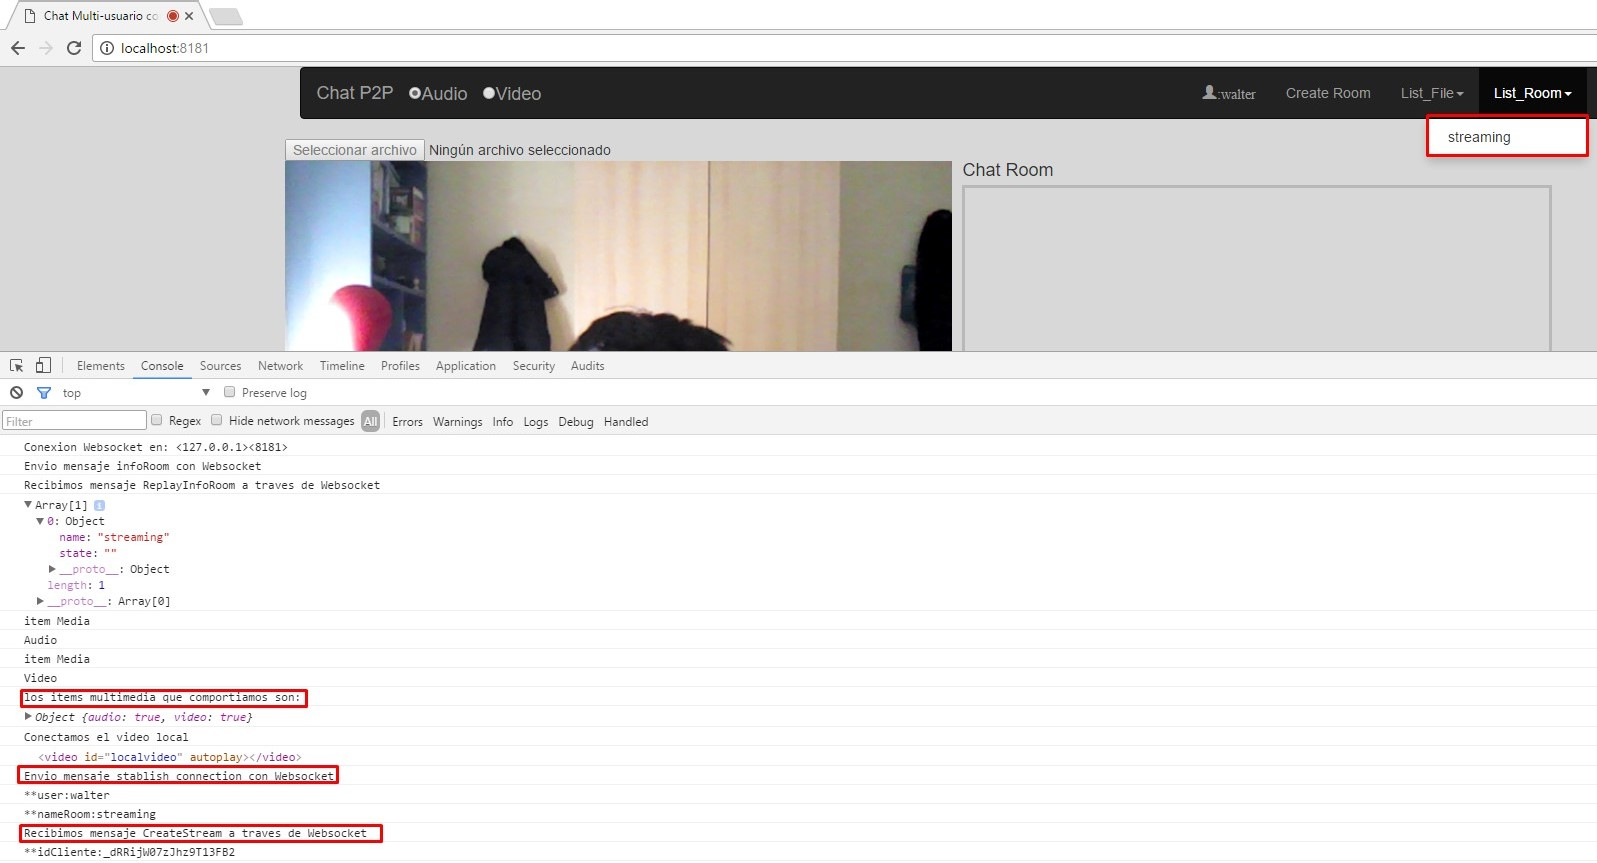
\includegraphics[width=1\linewidth]{Figures/StablishConnectionClient}
\decoRule
\caption[Inicio de conexión.]{Inicio de conexión.}
\label{fig:StablishConnectionClient}
\end{figure}
\subsection*{Proceso señalizacion WebRTC}
A partir del ultimo mensaje empieza el proceso de señalización que se divide en tres etapas: Oferta, Respuesta y Icecandidate. Es necesario definir la configuración del protocolo ICE en la variable \texttt{pc\_config} antes de iniciar este proceso.
\begin{lstlisting}[
caption=Configuración del protocolo ICE.]
 var pc_config = {'iceServers': [{'url': 'stun:stun.l.google.com:19302'}]};
\end{lstlisting}
%%%%%%%% Cliente offert %%%%%%%%
\subsubsection*{Ofera}
La función \texttt{create\_connection} inicia el proceso de oferta generando la instancia del objeto \texttt{RTCPeerConnection()} con la configuración del protocolo ICE definida en la variable \texttt{pc\_config}. Además vincula el flujo de vídeo local y el remoto a través del método \texttt{addStream()} y del evento \texttt{onaddstream}.

También define el canal de datos a través del método \texttt{createDataChannel} con los eventos necesarios para trabajar con este canal. Por ultimo genera la oferta a través del método \texttt{createOffer()} guardando su descripción de sesión con el método \texttt{setLocalDescription} y enviando este mensaje al nuevo usuario.
\begin{lstlisting}[
caption=Vinculamos vídeo local/remoto a RTCPeerConnection.]
 function create_connection(id){
  var pc = new RTCPeerConnection(pc_config,{});
  var num_user = 'user_'+ list_user.length;
  new_remote(num_user);
  pc.addStream(streaming);
    
  pc.onaddstream = function(event){
   var video = document.querySelector('#'+num_user);
   if(webrtcDetectedBrowser == 'firefox'){
    video.mozSrcObject = event.stream;
   }else{
    video.srcObject = event.stream;
   }
   video.play();
  };
  
  var sendChannel = pc.createDataChannel("sendDataChannel",
      {reliable: true});
  list_send.push(sendChannel);
  sendChannel.onopen = ChannelOpen;
  sendChannel.onclose = ChannelClose;
  sendChannel.onmessage = ChannelReceive;
  
  pc.createOffer(function(sessionDescription){
   pc.setLocalDescription(sessionDescription);
   var message = create_msg(my_id,id_newUser,sessionDescription);
   socket.emit('message',message);
   },function(err){console.log(err);},{}
  );
  
  pc.onicecandidate = SendICecandidate;
  list_user.push({id:id_newUser,peer:pc,data:sendChannel});
}
\end{lstlisting}

La figura \ref{fig:OfferCliente} muestra la creación de los elementos mencionados anteriormente dentro del objeto \texttt{RTCPeerConnection}.
\begin{figure}[!h]
\centering
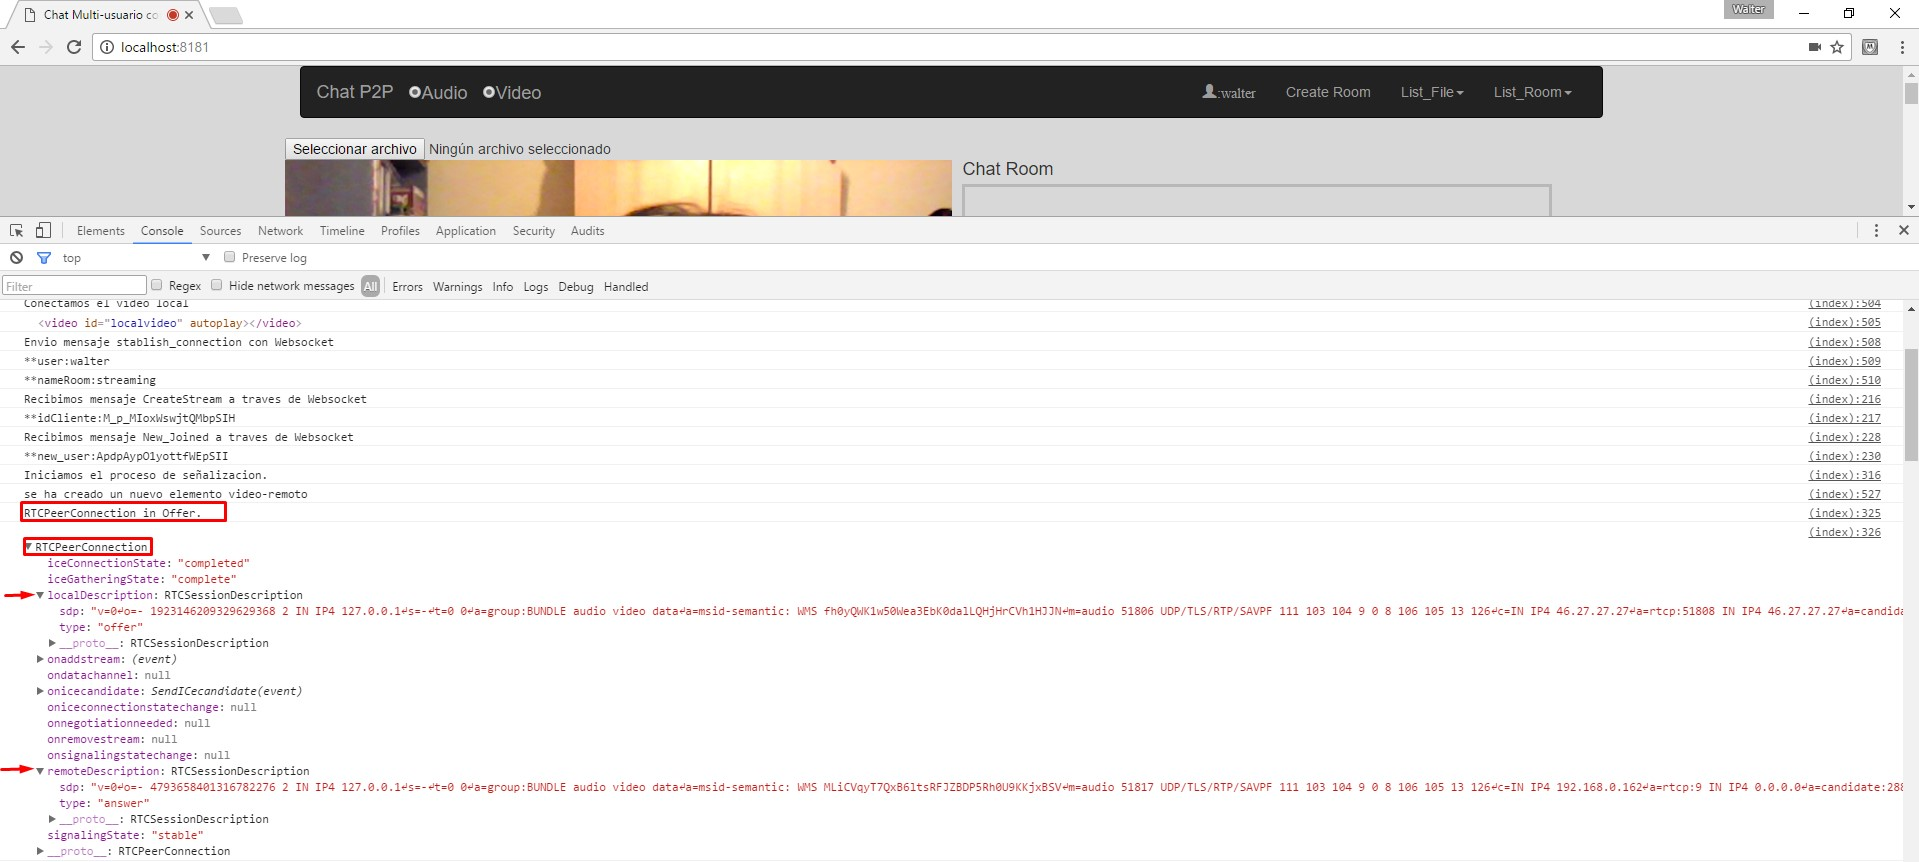
\includegraphics[width=1\linewidth]{Figures/OfferCliente}
\decoRule
\caption[Creación oferta cliente.]{Creación oferta cliente.}
\label{fig:OfferCliente}
\end{figure}

%%%%%%%% Cliente Answer %%%%%%%%
\subsubsection*{Answer}
EL otro usuario recibe un mensaje de oferta con la descripción de sesión del otro usuario. Al igual que en la oferta crea una instancia \texttt{RTCPeerConnection} en la que define los eventos \texttt{onaddstream}, \texttt{ondatachannel}, \texttt{onicecandidate}. Además crea un nuevo objeto \texttt{RTCSessionDescription} con la descripción recibida que se guarda como descripción remota por medio del método \texttt{setRemoteDescription}.

Finaliza creando el mensaje de respuesta con el método \texttt{createAnswer} añadiendo su descripción de sesión a través del método \texttt{setLocalDescription} y envía dicho mensaje al cliente.
\begin{lstlisting}[
caption=Recepción de la oferta.]
 if(message.message.type == 'offer'){
  var pc = new RTCPeerConnection(pc_config,{});
  id_newUser= message.id_origen;
  pc.addStream(streaming);
  pc.setRemoteDescription(new RTCSessionDescription(message.message));
  pc.onicecandidate = SendICecandidate;
  pc.onaddstream = function(event){
   var num_user = 'user_'+ list_user.length;
   new_remote(num_user);
   var video = document.querySelector('#'+num_user);
   if(webrtcDetectedBrowser == 'firefox'){
    video.mozSrcObject = event.stream;
  }else{
    video.srcObject = event.stream;
  }
  video.play();
  list_user.push({id:message.id_origen,peer:pc,data:receiveChannel});
 }
  pc.ondatachannel= function(event){
   list_send.push(event.channel);
   var receiveChannel = event.channel;
   receiveChannel.onmessage = ChannelReceive;
   receiveChannel.onopen = ChannelOpen;
   receiveChannel.onclose = ChannelClose;
  }
  pc.createAnswer(function(sessionDescription){
   pc.setLocalDescription(sessionDescription);
   var msg = create_msg(my_id,message.id_origen,sessionDescription);
   socket.emit('message',msg);
  },function(err){
   console.log(err);
  },{});
}
\end{lstlisting}

La figura \ref{fig:AnswerCliente} muestra como se crea la instancia \texttt{RTCPeerConnection} con los eventos que se han mencionado.
\begin{figure}[!h]
\centering
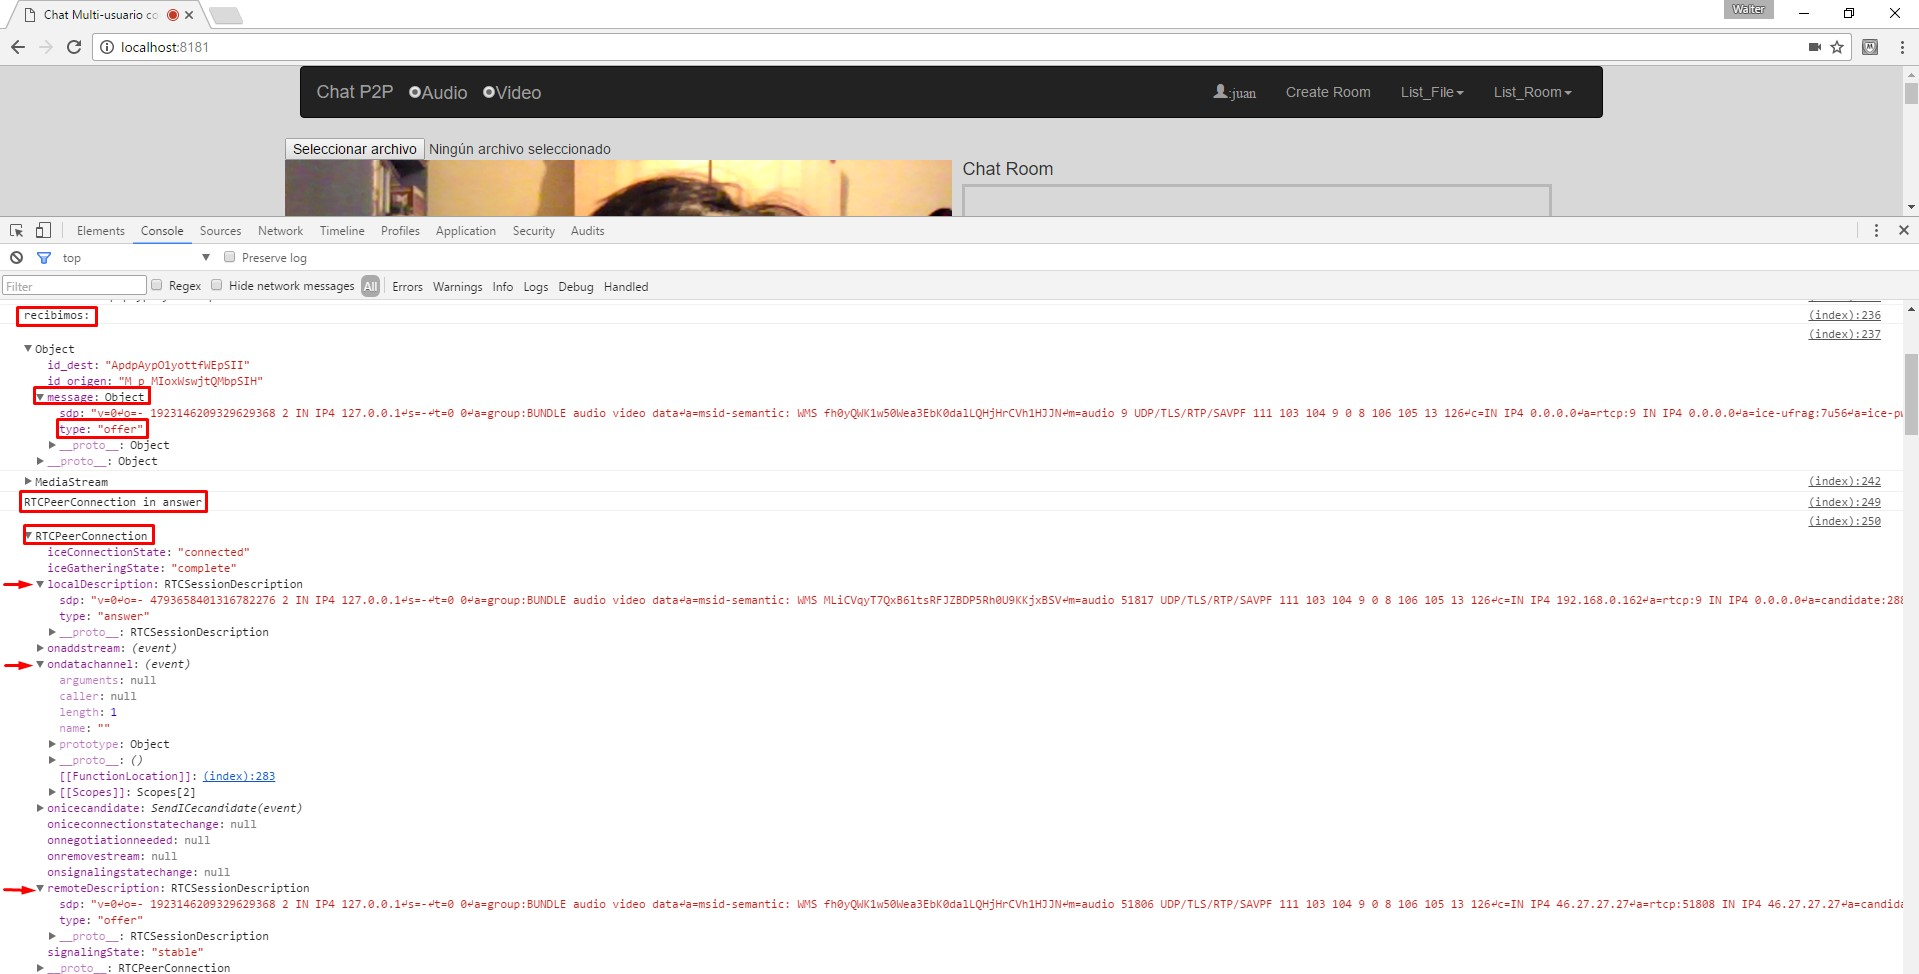
\includegraphics[width=1\linewidth]{Figures/AnswerCliente}
\decoRule
\caption[Creación de la respuesta.]{Creación de la respuesta.}
\label{fig:AnswerCliente}
\end{figure}

%%%%%%%% Cliente IceCandidate %%%%%%%%
\subsubsection*{Icecandidate}
Tanto el usuario local y como el remoto tras la generación del objeto \texttt{RTCPeerconnection} necesitan obtener información de la \texttt{Ip:Puerto} disponibles para la conexión por medio del protocolo ICE. Cuando se encuentra un candidato se ejecuta el evento \texttt{onicecandidate} que compone el mensaje con la información y lo envía a través de un mensaje de tipo \texttt{message}.
\begin{lstlisting}[
caption=Envió candidatos.]
 pc.onicecandidate = SendICecandidate;
 function SendICecandidate(event){
  if(event.candidate){
   var ice = {type: 'iceCandidate',
    label: event.candidate.sdpMLineIndex,
    id: event.candidate.sdpMid,
    candidate: event.candidate.candidate
   };
   var msg ={id_origen:my_id,id_dest:id_newUser,message:ice}
   socket.emit('message',msg);
  }
}
\end{lstlisting}

Los usuarios que reciben la información anterior generan un objeto \texttt{RTCIceCandidate} para llamar a la función \texttt{addIcecandidate} que se encarga de buscar dentro de la lista de conexiones la correspondiente y así guardar el objeto creado a través del método \texttt{addIceCandidate}.
\begin{lstlisting}[
caption=Recepción de candidatos.]
 var candidate = new RTCIceCandidate({
  sdpMLineIndex:message.message.label,
  candidate:message.message.candidate
 });
 addIceCandid(message.id_origen,candidate);
 function addIceCandid(id,message){
  for(var i=0;i<list_user.length;i++){
   var user = list_user[i];
   if(user.id == id){
    user.peer.addIceCandidate(message);
   }
  }
 }
\end{lstlisting}

Al conocer los usuarios la información de red y la descripción de sesión de cada uno esta etapa termina dando lugar a la conexión Peer-to-Peer.
\subsection*{Conexión WebRTC}
En esta etapa los usuarios intercambiando flujo de vídeo y audio en una conexión entre pares lo que permite que el canal de datos (\texttt{RTCDataChannel}) se encuentre operativo para enviar información por él como se describe a continuación.
\subsection*{Envió de cadena de texto}
A través del chat de la sala se puede enviar cadena de caracteres mediante la función \texttt{send\_data()}. La función genera un mensaje que contiene el flag \texttt{chat} y la cadena de texto para enviarlo por los distintos canales de comunicación disponibles. 
\begin{lstlisting}[
caption=Envió datos del chat.]
function send_data(elemento){
  var msg = $(elemento).val();
  var data = JSON.stringify({info:'chat',data:name+':'+msg});
  for(var i=0;i<list_send.length;i++){
   list_send[i].send(data)
  }
}
\end{lstlisting}
La figura \ref{fig:ChatClienteSend} es un ejemplo del envió de la cadena de texto tecleada por un usuario y enviada a los demás.

\begin{figure}[!h]
\centering
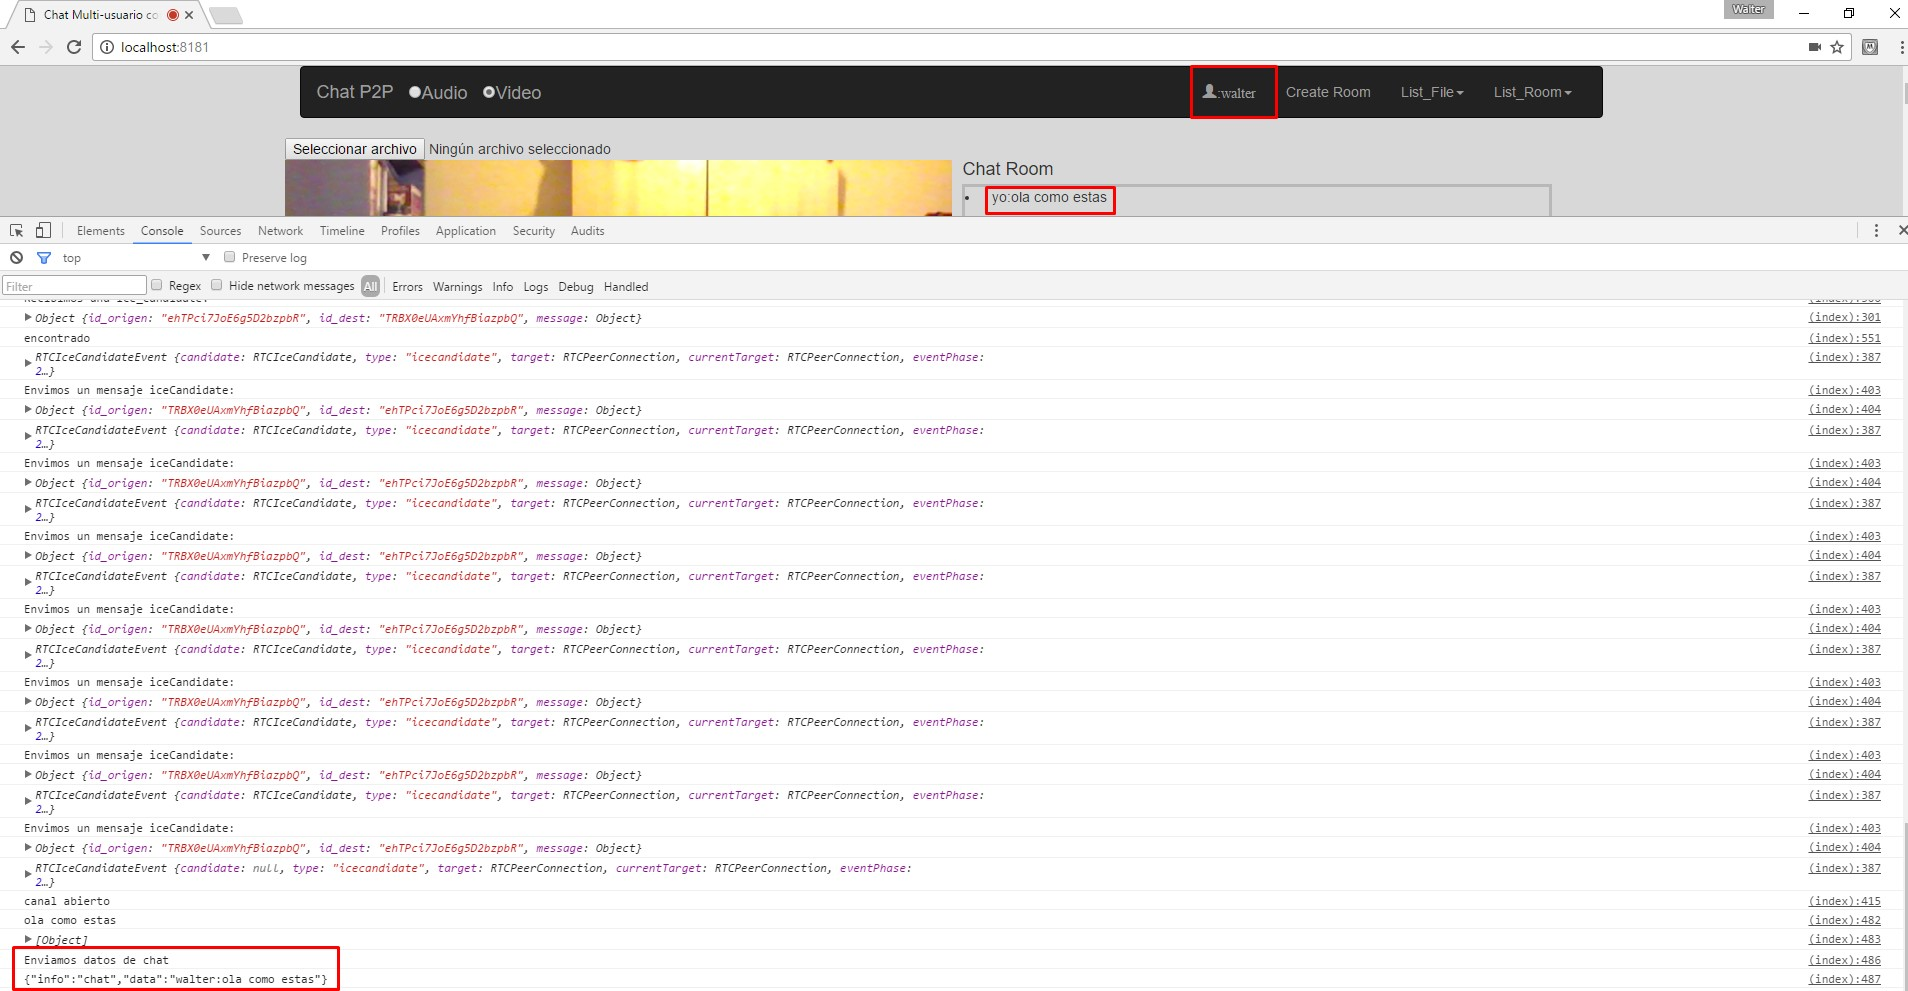
\includegraphics[width=1\linewidth]{Figures/ChatClienteSend}
\decoRule
\caption[Envió de caracteres del chat por RTCDataChannel.]{Envió de caracteres del chat por RTCDataChannel.}
\label{fig:ChatClienteSend}
\end{figure}

La recepción se realiza por medio de la función \texttt{WriteChat(\_data)} que se encarga de presentar dentro del chat la información que se ha recibido de otro usuario.
\begin{lstlisting}[
caption=Recepción datos del fichero.]
function WriteChat(_data){
 var line = document.createElement('li');
 var textnode = document.createTextNode(_data.data);
 line.appendChild(textnode);
 $('#texto').append(line);
}
\end{lstlisting}

\subsection*{Envió de ficheros}
Los usuarios disponen de un \texttt{input} de tipo file con el que carga el fichero que desea compartir. Tras seleccionar el fichero se ejecuta la función \texttt{processFiles(file)} que obtiene el contenido del fichero a través del objeto \texttt{FileReader()}. 
\begin{lstlisting}[
caption=Lectura del fichero.]
 function processFiles(file){
  var files = file[0];
  type = files.type;
  name_fich = files.name;
  var reader = new FileReader();
  reader.onload = function (e) {
   var data_file = reader.result;
   data_encript = arrayBufferToBase64(data_file);
   send_chucky();
  };
  reader.readAsArrayBuffer(files);
 }
\end{lstlisting}

El envió de los datos se realiza por medio de la función \texttt{send\_chucky()} en pequeños fragmentos de longitud fija ya que no sabemos la longitud del archivo y con el fin de no saturar el canal lo enviamos de esta forma. Cada envió esta formado por el flag \texttt{file} y el fragmento del archivo correspondiente, una vez se ha enviado se programa el siguiente envió mediante el evento timer \texttt{setTimeout(sendChuncky,time)}.

Al enviar el fragmento final del fichero se añade información adicional del fichero como el nombre y tipo de fichero ya que esta información es necesario para que el usuario receptor pueda reconstruir el fichero.
\begin{lstlisting}[
caption=Envió de fragmentos del archivo.]
 function send_chucky(){
  var last = false;
  fin = inicio + size_data;
  if(fin < data_encript.length){
   var data = JSON.stringify({info:'file',data:data_encript.slice(inicio, fin)});
   for(var i=0;i<list_send.length;i++){
    var user = list_send[i];
    user.send(data);
   }
   inicio = fin;
   setTimeout(send_chucky, 100);
  }else{
   last = true;
   var more_info ={type:type,name:name_fich};
   var data = JSON.stringify({info:'file',end:last,data:data_encript.slice(inicio, data_encript.length),more:more_info});
   for(var i=0;i<list_send.length;i++){
    var user = list_send[i];
    user.send(data);
   }
   inicio = 0;
  }
}
\end{lstlisting}
La figura \ref{fig:fildSendUser} muestra la obtención de información del fichero seleccionado y el envió de cada fragmento del fichero hasta finalizar.
\begin{figure}[!h]
\centering
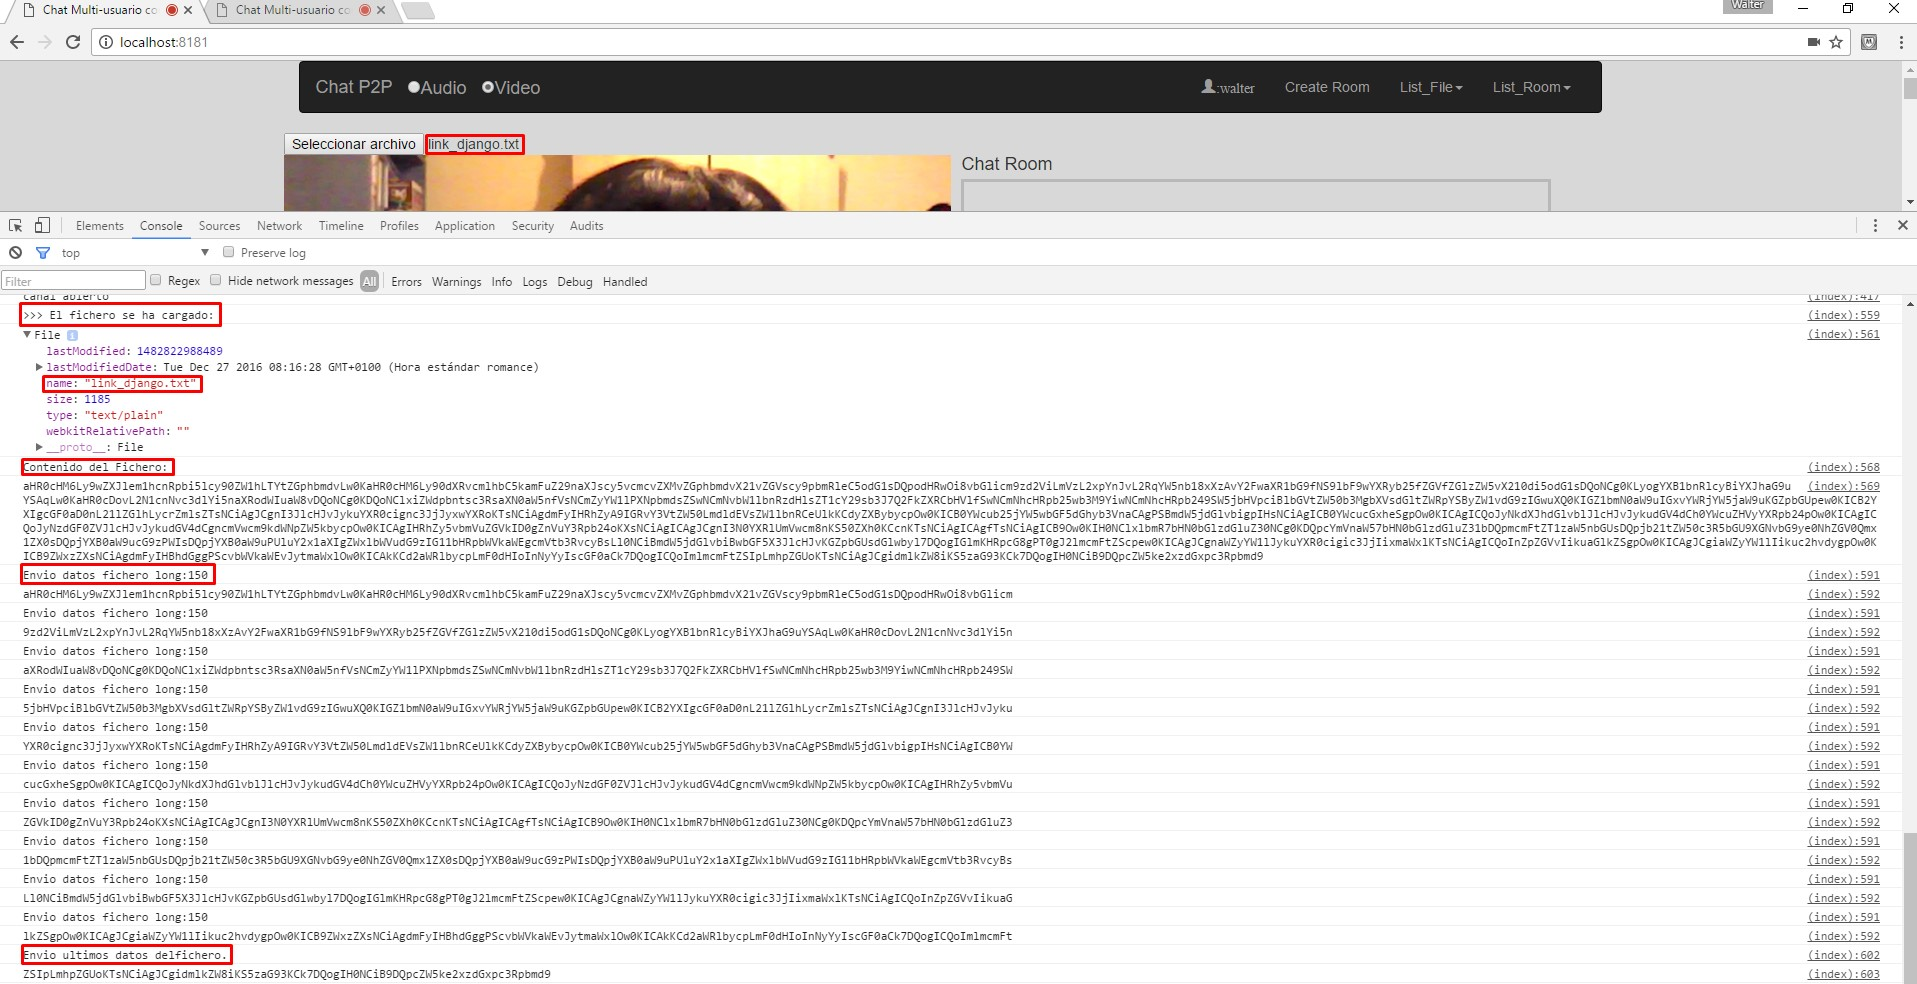
\includegraphics[width=1\linewidth]{Figures/filSendUser}
\decoRule
\caption[Envió información del fichero con  RTCDataChannel.]{Envió información del fichero con  RTCDataChannel.}
\label{fig:fildSendUser}
\end{figure}

El usuario receptor acumula cada uno de los fragmentos que recibe hasta obtener el ultimo fragmento mediante la función \texttt{BuildField()}. Al obtener el ultimo fragmento pasa a reconstruir el documento a través dentro de una etiqueta \texttt{<a>}, donde el atributo \texttt{href} esta formado por el tipo de archivo concatenado a los fragmentos del archivos.
\begin{lstlisting}[
caption=Recepción y reconstrucción del fichero .]
 function BuildFile(_data) {
  blob += _data.data;
  if(_data.end != undefined){
   if(_data.more.type == 'text/plain'){
    var link = document.createElement('a');
    link.href = 'data:'+_data.more.type+';base64'+blob;
    link.target = '_blank';
    link.download = _data.more.name;
    var textnode = document.createTextNode(_data.more.name);
    link.appendChild(textnode);
    $("#listFile").append(link);
   }
   blob =',';
  }
 }  
\end{lstlisting}

La figura \ref{fig:FieldReceiveUser} muestra la recepción de cada fragmento enviado por un usuario y la reconstrucción del fichero.
figur.
\begin{figure}[!h]
\centering
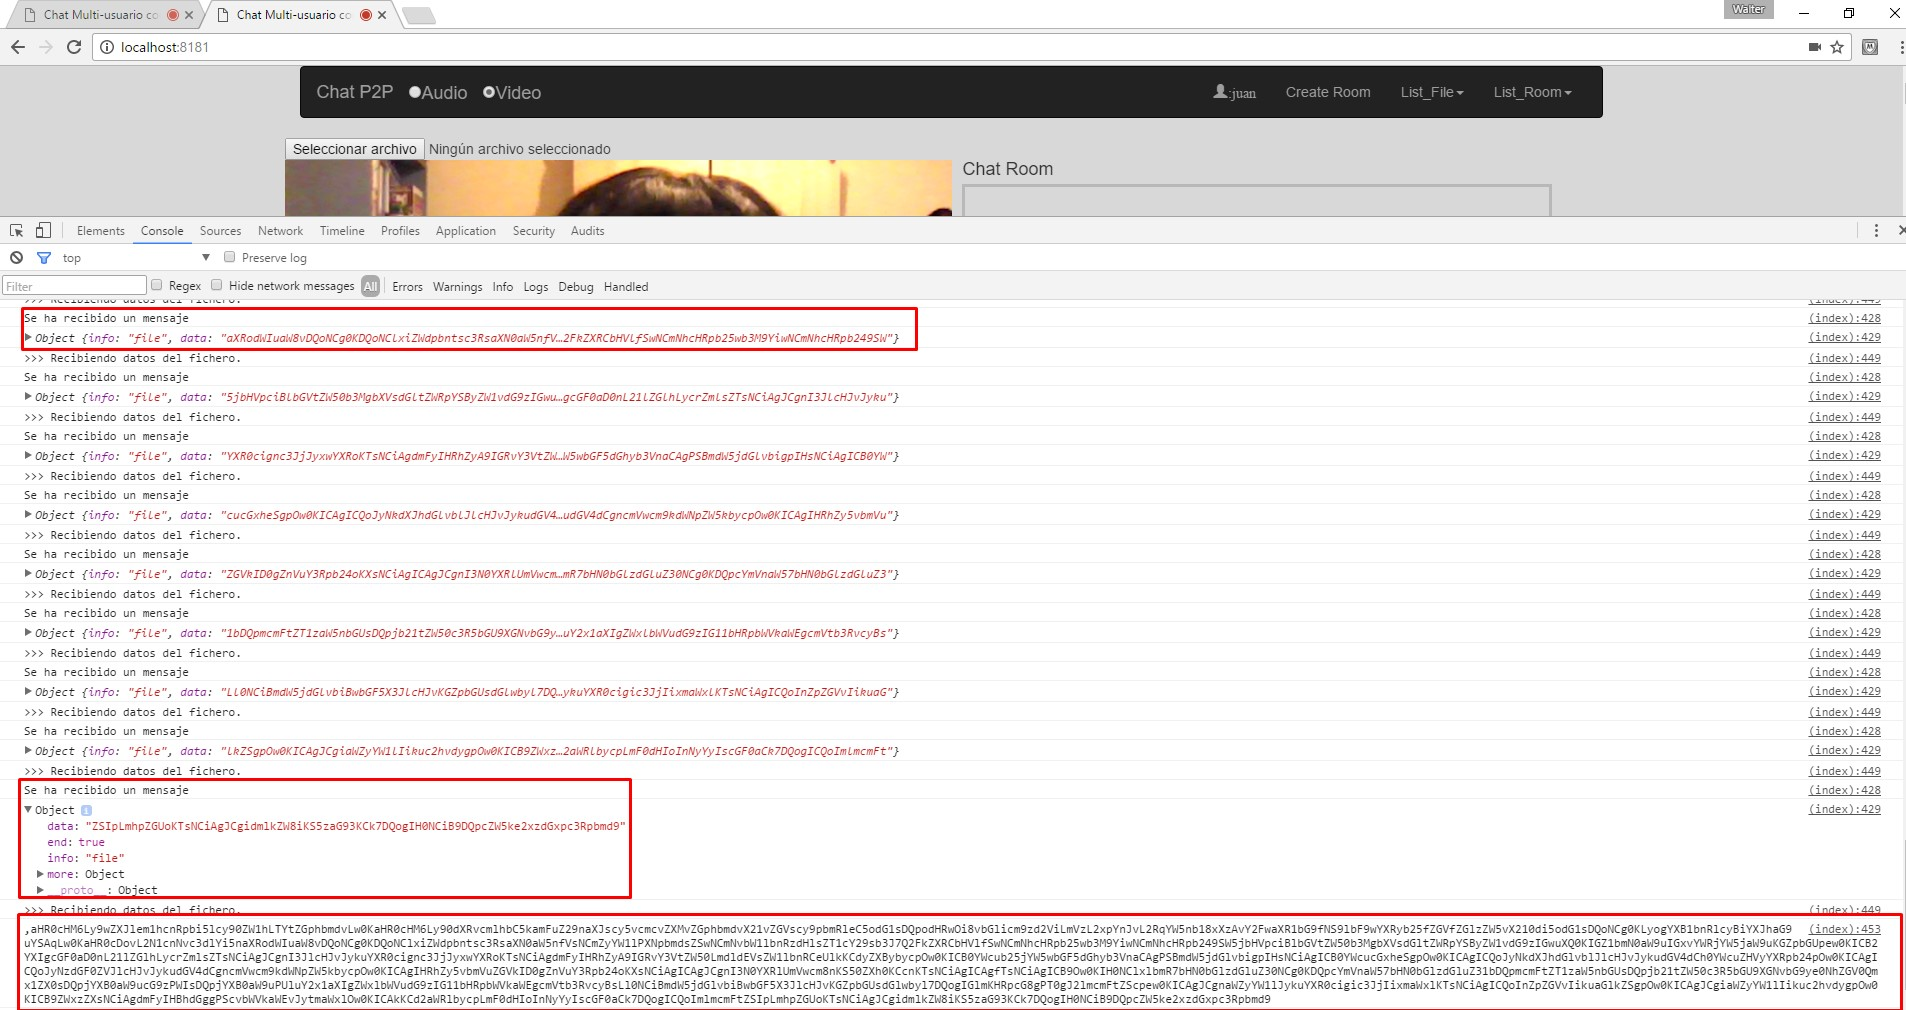
\includegraphics[width=1\linewidth]{Figures/filReceiveUser}
\decoRule
\caption[Recepción y reconstrucción del fichero]{Recepción y reconstrucción del fichero.}
\label{fig:FieldReceiveUser}
\end{figure}
